\documentclass{article}

\usepackage[dvips]{graphicx}

\begin{document}
\title{Dasher Geometry and Dynamics}
\author{Philip Cowans}

\maketitle

\begin{figure}
\begin{center}
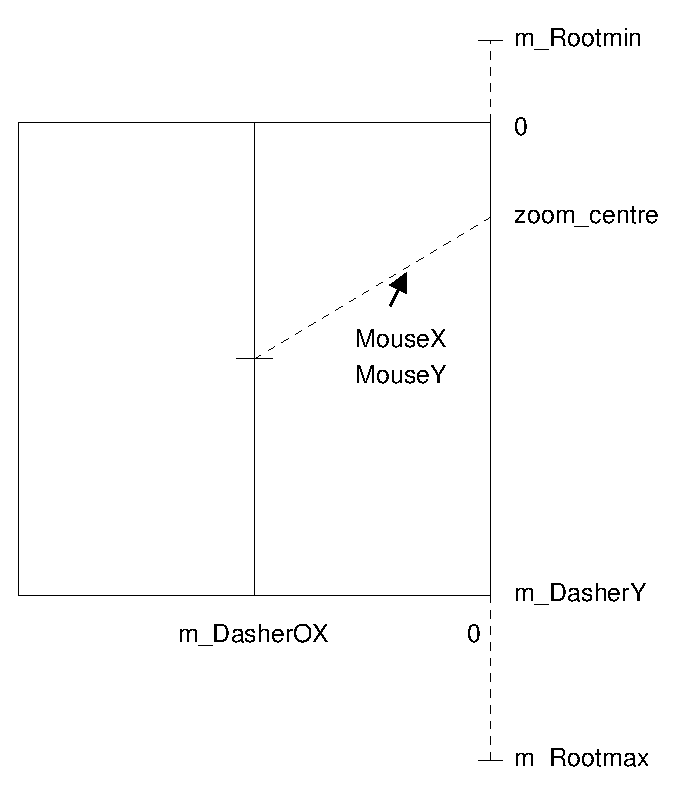
\includegraphics[height=8cm]{geometry}
\end{center}
\caption{Dasher geometry, showing variable names}
\label{geometry_fig}
\end{figure}

\section{Co-ordinate Systems}

There are three co-ordinate systems used in Dasher:

\begin{enumerate}
\item {\bf World Co-ordinates} Specifies the positions of the boxes on the Dasher world - the static sheet into which the user zooms. Co-ordinates are specified relative to the parent box. TODO: How are these stored etc?
\item {\bf Dasher Co-ordinates} Co-ordinates relative to the idealised Dasher viewport. $x$ co-ordinates are specified right to left\footnote{Dasher Co-ordinates are the same regardless of the display orientation, with the rotation done in the Dasher to screen co-ordinate mapping. In this guide I shall use the left-to-right conventions}, with the origin being to the right of the screen. They are scaled so that the cross-hair is at {\tt m\_DasherOX}. $y$ co-ordinates are specified top to bottom, with the origin being the top of the viewport and scaled so that the bottom of the viewport is at {\tt m\_DasherY}. See Figure \ref{geometry_fig} for a pictorial representation.

World co-ordinates are converted to Dasher co-ordinates by the notion of a root node whose upper and lower extremes have Dasher co-ordinates given by {\tt m\_Rootmin} and {\tt m\_Rootmax} respectively. Children of the root node can be located in Dasher space by recursively taking subintervals of this range. To prevent integer values from getting to large, one of the descendents of the root node is periodically promoted to the root, with the tree above this point being discarded. {\tt m\_Rootmin} and {\tt m\_Rootmax} are scaled appropriately at this point.

\item {\bf Screen Co-ordinates} These are the actual screen locations. As well as the appropriate scaling and translation, a non linear transformation is also applied in order to reduce the vertical size of the boxes near the top and bottom of the viewport.

\end{enumerate}

In the following, co-ordinates will be assumed to be in Dasher co-ordinates unless explicitly stated.

\section{Dynamics}

Dasher makes discrete updates to the display in order to zoom in on a chosen string. The underlying idea is that if the mouse is not further moved, the point in the Dasher world directly under the mouse cursor should move so that after a specific time it is under the cross-hair. 

This is achieved by zooming about the point on the right-hand edge of the viewport found by extending a line which passes through the cross-hair and the mouse cursor. The $y$ co-ordinate of this point is stored in {\tt zoom\_centre} (see Figure \ref{geometry_fig}).

To calculate the scale factor at each time step, first of all the scale factor required to place the point under the pointer under the cross-hair is calculated. The number of steps over which this should be done is also found. The latter is dependent on a number of factors, including the speed of the machine and the user-specified maximum bit rate and is stored in {\tt iSteps}.

Strictly speaking a geometric progression should be used to calculate a constant scale-factor for all steps in the series. In practice this is difficult to achieve using integer arithmetic, so an approximation is used instead (in the present implementation a linear division of the overall scale-factor is used, although a Taylor expansion around $1$ could give more accurate results if needed).

Having calculated the point about which to zoom, and the scale factor for the next time-step, it is straightforward to calculate the new values of {\tt m\_Rootmin} and {\tt m\_Rootmax} to reflect the enlargement of the root node.

\subsection{Notes}

There are a few issues which need to be taken into account when implementing the dynamics:

\begin{enumerate}
\item There are two singularities: at $x=0$ the scale factor becomes infinite. This is inherent in the definition of the dynamics and is solved by requiring that $x \geq 1$. There is also a singularity where the $x$ co-ordinate is aligned with the cross-hair, as in this case {\tt zoom\_centre} is the point at infinity. This is resolved by adding one to the $x$ co-ordinate in this position.
\item {\tt m\_Rootmin} and {\tt m\_Rootmax} must not be allowed to get so large that they overflow their data types. In practice this is almost always achieved by resetting the root before this is an issue, but in pathological cases this may not be possible, for example if a child of the root is sufficiently small that the root node gets too large before the child can be unambiguously selected (and therefore made into the new root). A solution to this problem, which is not explicitly implemented, is to require that the language model returns either zero or a value greater than some minimum chosen to prevent this ever being the case. Practically this could be achieved by appropriately setting the integer normalisation of the probability distributions.
\item If the user backs out too far, it may be possible to `loose' the root node, either off the side of the viewport or if it gets too small. This is currently prevented by requiring that the root is larger than one quarter of the height of the viewport, and that it crosses the mid-point of the right hand side.
\end{enumerate}

\subsection{An Alternative Representation}
\begin{figure}
\begin{center}
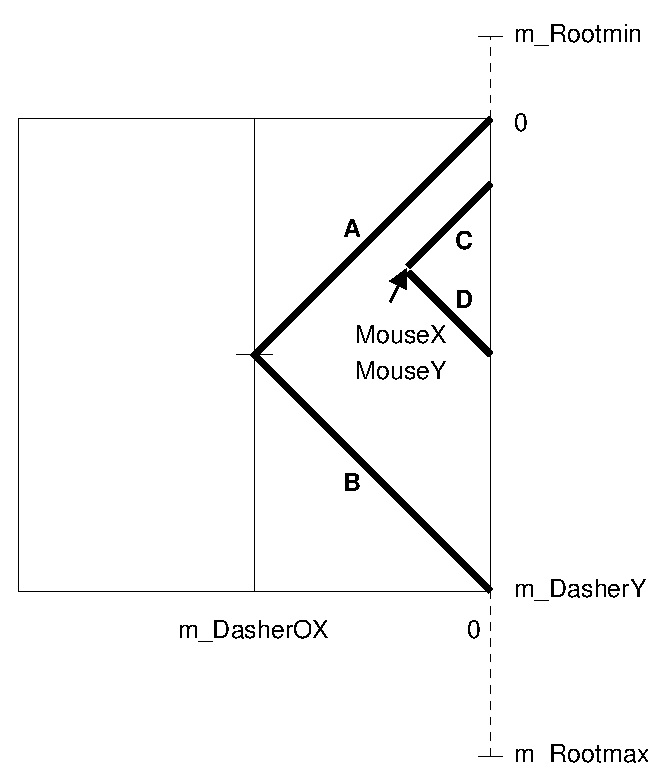
\includegraphics[height=8cm]{geometry2}
\end{center}
\caption{An alternative representation of the Dasher dynamics}
\label{geometry_fig2}
\end{figure}

Figure \ref{geometry_fig2} shows an alternative representation of the Dasher dynamics. In the diagram, lines A and C are parallel, as are B and D. The space enclosed by CD will become the full height of the viewport in {\tt iSteps} time-steps.

While functionally equivalent to the above, it may be better to represent things internally in this way and separate `calculate which update to do' from `update the root co-ordinates appropriately'. This should make a pure integer implementation easier, and will allow the latter to be shared with the various button input modes, for example allowing easy code re-use when deciding when re-parenting is necessary.
\end{document}
